\section{How does git work internally?}\label{howdoesgitwork}

To understand how git works we need to know some basic commands.

\subsection {Basic local commands}

As any other VCS git stores its data in the repository directory.
There are two major ways to get a repository.
One would be by simply creating a new empty git repository in your directory of choice:
\begin{lstlisting}
$ git init
\end{lstlisting}
This command creates a new subdirectory .git/ where all your version control
data is stored. \cite{gitinternals2008} p 55 \\
The second is to clone an existing repository over an URL. Possible protocols
are FILE SSH HTTPS HTTP or GIT. Of course on the target location must host a
git repository:
\begin{lstlisting}
$ git clone 
    git://github.com/rails/rails.git
\end{lstlisting}
Git will clone the whole ruby on rails project from github and we're
ready to get to work. \cite{gitinternals2008} p 56 \\

After we have a new repository we can add some content:
\begin{lstlisting}
$ touch README
$ git status
$ git add README
$ git commit -m "Added README file"
\end{lstlisting}

This code produces an empty README file. The status command displays any change
of the repository. There we can see that the README file has been added and we
track this file simply by telling git to add the file to the index. Additionally
git now stages the file, but we are going to cover the staging feature later in the next
section. Then we commit the changes with a short and descriptive message. After
this git stores the changes into the repository and points the default master
branch to the new commit. \cite{gitinternals2008} p 55 \\

\subsection {History}

With every commit Git will append information to the history of your project. This history
can be browsed using the \emph {git log} command:

\begin{lstlisting}
$ git log
commit 8133a...
Author: User <user@provider.org>
Date:   Wed Nov 17 19:29:03 2010 +0100

    [commit message]
    
commit 3131f...
Author: User <user@provider.org>
Date:   Wed Nov 17 19:29:03 2010 +0100

    [commit message]
    
...
\end{lstlisting}

Each commit consists of 4 parts: the commit SHA1 string, the author with his e-mail address, the commit date and a short descriptive message.
But this is not all you can see in the history. With several additional commands you can format the history or even display all the changes.
As an example this code formats the history quite different:

\begin{lstlisting}
$ git log 
   --pretty=format:"%h, %ar : %s"
8133ae1 4 days ago : fix issue 8645
741a1bc 4 days ago : merged crazyidea
3131fd0 4 days ago : added scripts
\end{lstlisting}

There are several more formating place holders that can be found at: http://progit.org/book/ch2-4.html.
\footnote{\cite{gitpro2009} http://progit.org/book/ch2-3.html on 21.11.2010}\\

As an example for the capability of the log command, there is a shell script\footnote{https://github.com/d1rk/git-ftp on 21.11.2010} on GitHub that allows you to upload your git repository over the ftp protocol. This script uses the git log command to get enough information to upload the changes to the ftp-server. 

\subsection{Git over network}

After there has been committed a huge amount of work in the local ruby on rails
repository we can share the work telling git:

\begin{lstlisting}
$ git push origin master 
\end{lstlisting}

This command will only succeed if you have the appropriate access rights to the
project. But if we had them, the master parameter tells git to take the default
branch and transmit the changes to the host. We could also specify any other
branch and transmit it to the destination host. \\ 

Also one should know that the origin parameter is our destination. You can
simply add many different socalled remotes:

\begin{lstlisting}
$ git remote add [name] [url]
\end{lstlisting}

This command links a short name to any url and you can share your
work over any network git is designed for. \cite{gitpro2009} chapter 2.9 \\

The last very important command is:
\begin{lstlisting}
$ git fetch origin
\end{lstlisting}

The fetch command is used to get work from other people of your project since
the last time you fetched. Very important is that this command does not
automatically merge the new updates into your local master branch. It just
downloads the updates and creates a new brach FETCH\_HEAD. Then you have to
manually merge the branch FETCH\_HEAD to the desired branch. 
If you dont need this very powerful feature you can simply execute:
\begin{lstlisting}
$ git pull origin
\end{lstlisting}
Git will automatically merge the changes into your master branch.
\cite{gitpro2009} chapter 2.9 \\

\subsection {Staging}

Now that we convered the fundamental basics of git. We can take a deeper look at
some parts of the logic used by git. One high level feature of git is the
\emph{interactive adding}. We create a new repository and add a file and commit
it. If we modify the same file again and try to commit with the command above,
git will not apply the modified file to the repository. This is because this file is
not explicitly added to the socalled staging mode. You have to explicitly add
the modified file to the staging mode and commit. This feature gives you much
more control over what goes into your repository or not. This feature is often
ignored and you can simply commit a unstaged file with this command:

\begin{lstlisting}
$ git commit -a -m "message"
\end{lstlisting}

The parameter \emph{-a} automatically adds the file to the staging mode and
commits it. \cite{gitpro2009} chapter 2.2

The picture\footnote{http://progit.org/figures/ch2/18333fig0201-tn.png last accessed on 
09.11.2010} taken out of the git pro book illustrates how files change their
lifecycle modes:

\begin{figure}[h]
  \centering
  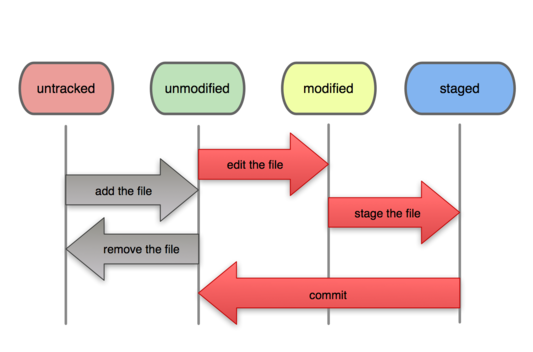
\includegraphics{img/file_status_lifecycle}
  \caption{File status lifecycle}
  \label{fig:File status lifecycle}
  
\end{figure} 

As we can see there are four modes a file can have. First we have to track them
once to get them into the lifecycle. If we modify we can use \emph{-a} on the
commit command to automatically stage and commit them, or we can take alot more
control of our repository and stage them manually and avoid mistakes and
redundant changes that do not belong to a certain commit.
We can simply get information about the mode using the git command
\emph{status}. \cite{gitpro2009} chapter 2.2

\subsection{How does git store its data?}
Git uses a unique store model compared to other common DVCS like Baazar or Mercurial. 
In tradional distributed or normal version control the system keeps differences between revision A and B. 
These changes are saved and marked with a revision number. 
So you can, at any time, switch back to any revision and rebuild the complete content.
This does have some major downsides which we will see later. \\
Git does handle it quite different. It takes socalled \emph{snapshots} in every
new version. So if file A changes in your repository the next commit git will take a new snapshot of this file and all other files. 
To reduce overhead not changed files are linked to the identical file in the previous verion. 
It creates a new minifile system rather than a VCS, enabling you all the features normal version 
control would give you and gives you some additional on top of it. \cite{gitpro2009} 

\subsection{Checksums for integrity}

\zitat{ Every single piece of data, when git tracks your content, we compress it
we delta it against everything else, but we also do a SHA1 hash of the content
and we actually check it when we use it. If you have discorruption if you have
dramcorruption if you have any kind problems at all git will notice them. It is
not a question of if, it is a guarantee } \cite{googletechtalk2007}

Git is secure. As you can see in Linus Torvalds speech, git uses the SHA1-Hash
as an integrity feature. Secure Hash Algorithm 1 is a string with 40 hexadezimal
characters. It creates a checksum of two pieces of data and makes it nearly
impossible that 2 files have the same checksum. This makes discorruption or loss
of data impossible without notice. \footnote{ \cite{gitpro2009} http://progit.org/book/ch1-3.html }

\subsection {Branching}

Branching is a major features in git. But also like the staging mode
branching can be skipped and you can just stick to the master
branch. \\
Assumed we have a new feature request for the ruby on rails project called
newfeature we add a branch:
\begin{lstlisting}
$ git branch newfeature
$ git checkout newfeature
\end{lstlisting}

To understand what branching do technically we have to take a deeper look at
what a commit does internally: \
After you execute the commit command Git creates a new commit object that
contains a pointer to the snapshot of your content you staged, some metadata and
pointers to you previous commits. If there are zero previous commits no pointer
is stored and if you merged a branch the commit can point to multible previous commits.

After staging a single file, Git creates a checksum (see
\ref{SHA1}) and stores the version in the repository. Additionally it adds the
checksum to the staging area. This file is now a blob object.
When you execute the commit command, Git will create checksums for each
subdirectory and adds this tree object to the repository. Finally git creates
the commit object that contains the metadata and a pointer to the root object
tree. This is necessary to be able to recreate the snapshot.

We have three new objects in our repository describing the part of the history
of the project. There is one blob for the file we staged, the tree object that
points to the blob and a commit object that points to that tree object including
all metadata, like commit message and author. 
\\

Lets see what the releationship between these objects look like:

\begin{figure}[h]
  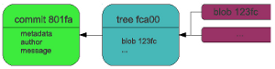
\includegraphics{img/branch2}
  \caption{Git objects after a commit}
  \label{fig: git objects after a commit}
  %\author{Richard Plangger}
\end{figure}

It is obvious that very commit looks like this and every commit, exept the first
has one or more parents.
A branch is just a moveable pointer towards a commit. Also the master branch is
one of those ligthweight pointers towards a commit. In addition there is a
pointer called HEAD which specifies which branch we are currently on. So by
executing the command \emph{git checkout [branchname]} we move the HEAD
pointer. 

Now it is time to make a new commit in the crazyidea branch and switch back to
the master branch and also commit some changes.
This could look like this:
\begin{figure}[h]
  \centering
  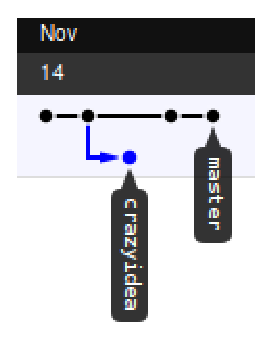
\includegraphics{img/branch3}
  \caption{The new branch crazyidea}
  \label{fig: a new branch}
\end{figure}

There has been created a new commit pointing to one commit of the master branch.
The new commit in its own branch now contains the history from the master branch
to the commit where it was splitted from and the changes in the new
branch. The last two commits that has been made in the masterbranch are not
visible in our new branch. 

Because a new branch in git is equal to a single
file with the SHA1 checksum branches are very cheap. In other version control systems branching means to
fully copy the whole content into a new folder and not just create a 41 byte big
file. This can take seconds or even minutes and discourages developers to use
this powerful feature. \footnote{ \cite{gitpro2009} http://progit.org/book/ch3-1.html }

\subsection {Merging}

Merging is the need of putting together data from different branches. Maybe one
day our crazy idea will turn out to be brilliant and also the crazyidea is
stable enough to put it to our master branch we need a way to put them together.
At this point the merge command pops in:

\begin{lstlisting}
$ git merge [branchname]
\end{lstlisting}

Git now merges all differences into the branch we're currently on and we can see
the result:
\begin{figure}[h]
  \centering 
  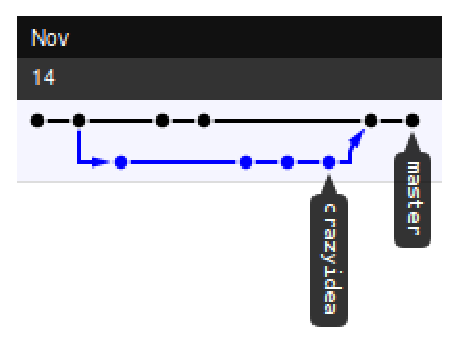
\includegraphics{img/merge1}
  \caption{Merged the crazy idea into the master branch}
  \label{}
\end{figure}

After the merge all data that is not contained in master but in crazyidea is put
together and will be part of master. As we can see this is very powerful feature
that allows developers to be flexible and work on several different parts of the
project, without breaking the whole project. \footnote{ \cite{gitinternals2008}
p. 30-31}

\subsection {What makes git to a DVCS?}

Linus Torvalds did a quite good job to summarize what distributed means:

\zitat{Being distributed very much means that you do not have one
central location that keeps track of your data, no single place more important
than any other place \ldots } \cite{googletechtalk2007}

Nearly all commands that git offer you are local operations. There is no need to
have any network connection at all to work on your project and track changes
afterwards. Moreover the whole history of your project is contained in your
local repository. Also all contributors of one project have that history if
they pull from you. Hence no repository has more information about the project
than the other.

